
\clearpage\section{スクレイピングで取得した情報を習った技術と組み合わせる}
これまでの例で、ウェブページをスクレイピングして、必要な情報を取り出す方法を学びました。
次は、スクレイピングを習った技術と組み合わせることを学びます。
スクレイピングだけでも、かなりできることは広がりますが、やはりセンサーボードやJulius、OpenJtalkなど習った技術と組み合わせるとさらに便利で楽しいものが作れます。

\refstepcounter{Exercise}
\clearpage\section{\theExercise スクレイピングした情報をもとにセンサーを使う}
\addtocounter{Exercise}{-1}\refstepcounter{Exercise}\label{E:amedasSensor}
スクレイピングで得た情報を習った技術(センサーボードの使い方、OpenJtalk,
Juliusなど)と組み合わせて便利なことや楽しいことをする練習をしましょう。
この例では、アメダスのウェブページから取得した気温を使って暑いか\ruby{涼}{すず}しいかを判断してLEDで通知してくれるプログラムを試します。
その後にこのプログラムを変更して、気温以外の情報を使用してより高度な通知ができるようにしてみましょう。

まずは、実行してみましょう。

ターミナルを開いて、

hsed

と実行してスクリプトエディタを開きます

\begin{center}
  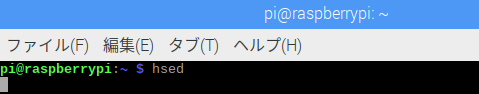
\includegraphics[width=\textwidth]{textbook-img013.png}
\end{center}
ファイル→開く をクリックして\textbf{{\textasciitilde}/08/amedas\_led.hsp}を開きます。

\begin{center}
  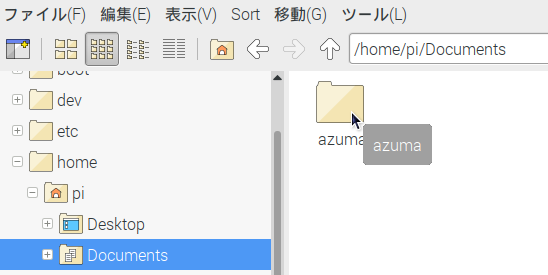
\includegraphics[width=12.173cm]{textbook-img038.png}
\end{center}

\clearpage
F5を押して実行してみましょう。

\begin{center}
  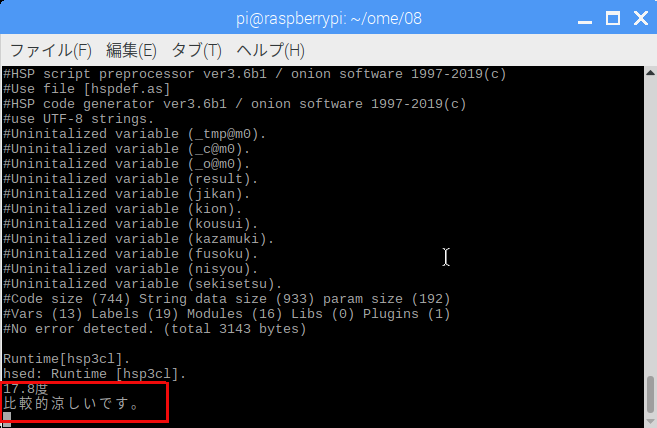
\includegraphics[width=\textwidth]{textbook-img039.png}
\end{center}
ターミナルには現在の気温と、判断した結果(暑いか涼しいか)が表示されます。

LEDに注目すると、暑いときには緑色のLED、涼しいときはオレンジ色のLEDで通知しています。

\clearpage
\noindent プログラム解説
\begin{center}
\begin{boxedminipage}{15.272cm}
\begin{enumerate}
\setlength{\itemsep}{0cm} % 項目間
\item \#include {\textquotedbl}hsp3cl.as{\textquotedbl}
\item \#include {\textquotedbl}cmdexec.as{\textquotedbl}
\item
\item cmdexec {\textquotedbl}amedas.py{\textquotedbl}, result
\item split result, {\textquotedbl},{\textquotedbl}, jikan, kion, kousui, kazamuki, fusoku, nisyou, sekisetsu
\item
\item mes kion + {\textquotedbl}度{\textquotedbl}
\item if int(kion) {\textgreater} 28 \{
\item \ \ mes
{\textquotedbl}気温が高いです。\ruby{熱中症}{ねっちゅうしょう}に注意しましょう{\textquotedbl}
\item \ \ gpio 17, 1
\item \ \ await 100
\item \ \ gpio 17, 0
\item \} else \{
\item \ \ mes {\textquotedbl}比較的涼しいです。{\textquotedbl}
\item \ \ gpio 18, 1
\item \ \ await 100
\item \ \ gpio 18, 0
\item \}
\item ; プログラムの終了
\item end
\end{enumerate}
\end{boxedminipage}
\end{center}


7行目までは\ref*{E:UTF8}と基本的に同じです。

8〜18行目で、温度をもとに暑いか、涼しいかメッセージを表示させてLEDを点灯させています。

8行目で

int(kion)としています。
kion変数は文字列で気温を入れているので、大小の比較はできません。

まずは、文字列から数値へ変換が必要です。

そのときに使うのがint関数です。

\begin{center}
\tablefirsthead{}
\tablehead{}
\tabletail{}
\tablelasttail{}
\begin{supertabular}{|m{16.806cm}|}
\hline
int関数の使い方

i = int(“12”)

文字列を数値へ変換してくれます。

i ← 12

int関数は小数点は扱えないので注意が必要です。
	小数点を扱いたい場合はdouble関数を代わりに使用します。

double関数の使い方

f = double(“12.3”)

f ← 12.3

f = double(“1”)

f ← 1.0\\\hline
\end{supertabular}
\end{center}


8行目で

if int(kion) {\textgreater} 28

kionを数値に変換して、28と大小の比較をしています。

28度より気温が高ければ暑い、それ以外では涼しいと判断します。

\refstepcounter{Question}
\subsection*{\theQuestion\label{Q:amedas4}}
\begin{itemize}
  \item 例題では気温を文字列から数値へ変換しましたが、変数へは値をいれていません。気温を数値へ変換して、結果を変数へ入れてみましょう。変数名はtempとしましょう。
\end{itemize}
\ \ HINT : temp = int(kion)

\ \ \ \ 気温(kion)を数値へ変換した値をtemp変数へ入れる。

\refstepcounter{Question}
\subsection*{\theQuestion\label{Q:amedas5}}
\begin{itemize}
  \item 現在の風速も表示するようにしてみよう
\end{itemize}


\clearpage
\refstepcounter{Question}
\subsection*{\theQuestion\label{Q:amedas6}}
\begin{itemize}
  \item 例題では、気温を使って比較をしました。次は風向きを使用して風が強いとき(15m/sより大きい)は”強風に注意しましょう”と表示をしてLEDを光らせましょう。それ以外の場合は”現在の風速”を表示して他の色のLEDを光らせましょう。
\end{itemize}
\refstepcounter{Question}
\subsection*{\theQuestion\label{Q:amedas7}}
\begin{itemize}
\item LEDだけでなくFaboなどのセンサーを使用して通知するようにしてみよう。
\end{itemize}
\ \ \ \ HINT : \ruby{振動子}{しんどうし}など

\refstepcounter{Question}
\subsection*{\theQuestion\label{Q:amedas8}}
\begin{itemize}
  \item センサーボードについている4つのLEDを使って、現在の温度を表すバーグラフを作ってみよう。(LEDを左から順に15, 20, 25, 30度のときに光るようにしてみよう。)
\end{itemize}
\ \ HINT:
LEDの色は左からLED1(緑)、LED2(黄)、LED3(青)、LED4(白)です。

\begin{center}
  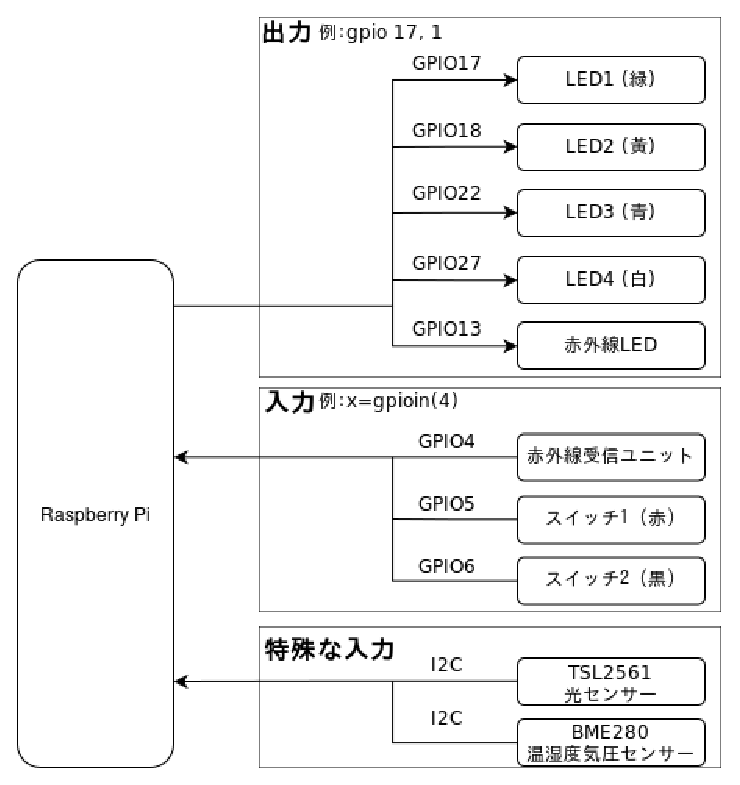
\includegraphics[width=0.6\textwidth]{textbook-img040.eps}
\end{center}

\refstepcounter{Exercise}
\clearpage
\section*{\theExercise TV番組表のウェブページをスクレイピングする}
\addtocounter{Exercise}{-1}\refstepcounter{Exercise}\label{E:TV}
\noindent 考え方

まずは、ウェブブラウザでTV番組表のページを見てみよう。
授業で使用したホームページを開いてください。
\textbf{({\textasciitilde}/08/links.html)}

TV番組表をクリックします。

\begin{center}
  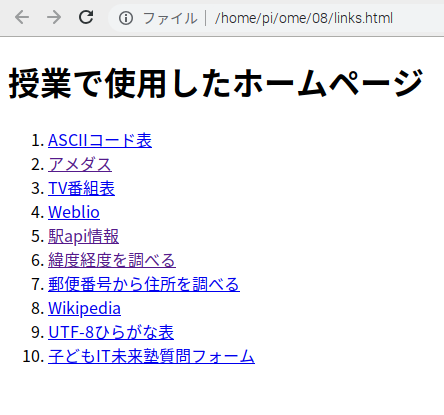
\includegraphics[width=0.6\textwidth]{textbook-img017.png}
\end{center}

TV番組表のウェブページが開きます。
このページの\ruby{検索欄}{けんさくらん}に検索したいワードを入れて検索をすると結果がでてきます。
まずは、\ruby{適当}{てきとう}に検索してみましょう。
\begin{center}
  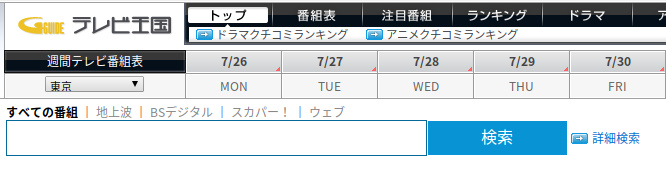
\includegraphics[width=0.85\textwidth]{textbook-img041.png}
\end{center}

\clearpage
試しに”サザエさん”と検索してみました。
結果の画面はこのような感じです。
TVの番組なので検索したタイミングによって番組がやっていなかったりしますのでそのような場合は検索ワードを変更してください。

\begin{center}
  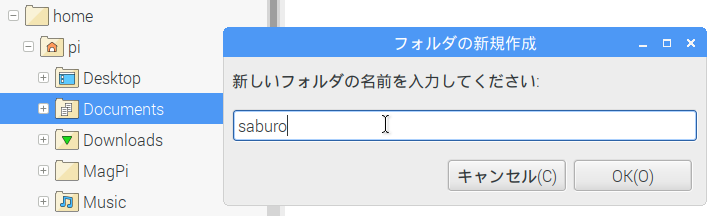
\includegraphics[width=\textwidth]{textbook-img042.png}
\end{center}
今回取得する情報は、検索ワードに対応する検索結果のタイトルと日付です。

まずはプログラムを動かしてみましょう。

ターミナルを開いて

hsed

と実行してスクリプトエディタを開きます。

\begin{center}
  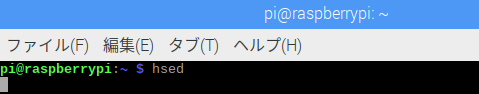
\includegraphics[width=\textwidth]{textbook-img013.png}
\end{center}

\clearpage
HSPスクリプトエディタが開くので

ファイル → 開く..\ をクリックして\textbf{{\textasciitilde}/08/tv.hsp}を開きます。

プログラムが表示されます。

\begin{center}
  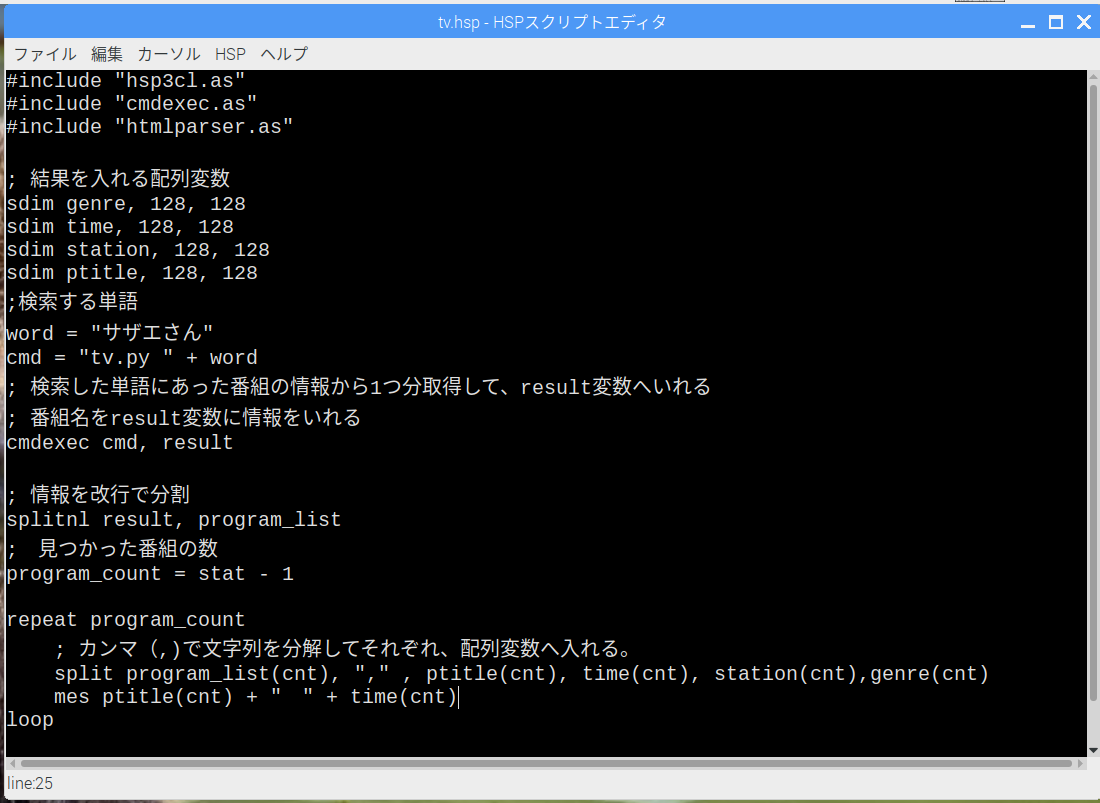
\includegraphics[width=0.85\textwidth]{textbook-img043.png}
\end{center}

F5を押して実行してみましょう。

実行結果はターミナルに表示されます

\begin{center}
  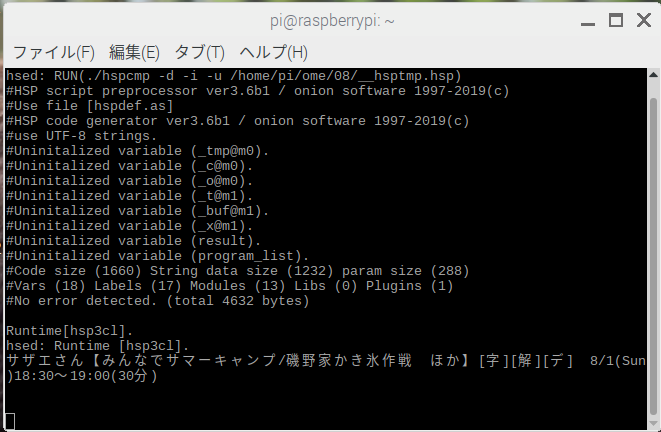
\includegraphics[width=0.85\textwidth]{textbook-img044.png}
\end{center}

ブラウザの表示とプログラムの実行結果を比べてみてください。
実行結果では日付と番組名だけ表示しています

\begin{center}
  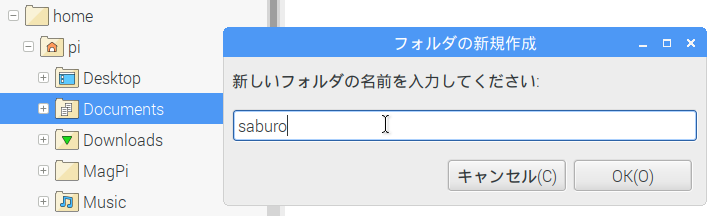
\includegraphics[width=0.85\textwidth]{textbook-img042.png}
\end{center}

\subsection*{}
\refstepcounter{Question}
\subsection*{\theQuestion\label{Q:TV}}
6行目のword=”サザエさん”で検索する番組を指定しています。
自分の検索したい番組名にして実行してみましょう。

\refstepcounter{Question}
\subsection*{\theQuestion}
このプログラムでは、日付(date配列)と番組名(ptitle配列)しか表示をしていません。
ジャンル(genre配列)とテレビ局(station配列)を表示するようにしてみましょう。
